% !TEX root = ejb-web.tex
%!TEX encoding = UTF-8 Unicode
\ifx\setbeamertemplate\undefined
\documentclass[handout]{beamer}
\fi
\graphicspath{{../images/}}
\usepackage{amsmath}
\usepackage{xifthen}

\usepackage{mathtools}
\mathtoolsset{showonlyrefs}
\usepackage{mathrsfs}

\usepackage[multidot]{grffile}

\usepackage{xspace}
\usepackage{upgreek}
\newcommand\xsb{$\upchi$SB\xspace}
\newlength{\imagecolumnwidth}

\usepackage[absolute,overlay]{textpos}

\usepackage{slashed}
\newcommand\dslash{\slashed{\partial}}

\usepackage{bbold}
\newcommand\one{\mathbb{1}}

\usepackage{multirow}

\newcommand\bs\boldsymbol

\newcommand \Sx[1] {S_{\textnormal{#1}}}
\newcommand \Sg[2] {\mathrm{#1}(#2)}
\newcommand \SU[1] {\Sg{SU}{#1}}
\newcommand \SO[1] {\Sg{SO}{#1}}
\newcommand \Sp[1] {\Sg{Sp}{#1}}
\newcommand \Uone {\Sg{U}{1}}

\newcommand\pb{\overline{\psi}}
\newcommand \bigL {\mathscr{L}}
\newcommand \lag[1] {\bigL_{\mathrm{#1}}}

\newcommand\sptn{Sp($2N$)\xspace}
\newcommand\dee{\mathrm{d}}
\newcommand\eee{\mathcal{E}}
\newcommand\www{\mathcal{W}}
\DeclareMathOperator\tr{tr}
\DeclareMathOperator\real{Re}
\newcommand\Nf{N_{\mathrm{f}}}

%\usepackage{beamerthemesplit} %Activate for custom appearance
\setbeamertemplate{navigation symbols}{}%remove navigation symbols

\usefonttheme[onlymath]{serif}
\usepackage{fontspec,xltxtra,xunicode}
\defaultfontfeatures{Mapping=tex-text}
\setsansfont[Scale=MatchLowercase,Mapping=tex-text]{Futura}
\setbeamerfont{structure}{family=\fontspec{Cosmos BQ}}
\definecolor{swanseablue}{RGB}{36,47,96}
\setbeamercolor{structure}{fg=swanseablue}
 \setbeamertemplate{itemize item}{•}
 \setbeamertemplate{itemize subitem}{--}
 \setbeamercolor{itemize item}{fg=black}
 \setbeamercolor{itemize subitem}{fg=black}

\newcommand\disappear[1]{}
\title{Beyond \texttt{MPI\_Send}: What I learned implementing MPI for halo exchange}
\author{{\large Ed Bennett}
	\\{\small@QuantumofEd}
	\\\vspace{16pt}
	\hfill
	\parbox{0.22\textwidth}{\centering
\includegraphics[height=36pt]{logos/swansea}\\\small @SwanseaUni}
	\parbox{0.44\textwidth}{\centering
\includegraphics[height=24pt]{logos/scw}\\\small @SuperCompWales}
	\parbox{0.22\textwidth}{\centering
\includegraphics[height=36pt]{logos/sa2c}\\\small @sa2c\_swansea} }
\date{SA2C Tech Chat, 2018-07-27}

\newcommand\Wider[2][3em]{%
\makebox[\linewidth][c]{%
  \begin{minipage}{\dimexpr\paperwidth-#1\relax}
  \raggedright#2
  \end{minipage}%
  }%
}



\newcommand\FrameText[1]{%
  \begin{textblock*}{0.9\paperwidth}(3pt, 0.99\textheight)
    \raggedright #1\hspace{.5em}
  \end{textblock*}}

\newcommand \sechead[1] {\frame{\vfill\Huge \centering\usebeamerfont{structure}\color{swanseablue}#1\vfill\null}}

\usebackgroundtemplate%
{%
	
\includegraphics[width=\paperwidth,height=\paperheight]{background/bg}%
}
\setbeamertemplate{footline}{
	\vspace{1.0cm}
}


  
\begin{document}

\frame{\titlepage}

\begin{frame}[fragile]{Background}
	\begin{itemize}[<+->]
		\item Lattice field theory code
		\begin{itemize}[<+->]
			\item Originally in FORTRAN IV/77
			\item Using \verb|-parallel| scaled well to 4 threads
			\item Refactored to Fortran 90ish
			\item Indirection replaced with explicit indexing
			\item All arrays have static sizes
		\end{itemize}
		\item Three-dimensional problem; 1-3 additional d.o.f.s
	\end{itemize}
\end{frame}

\begin{frame}{3D lattice}
	\center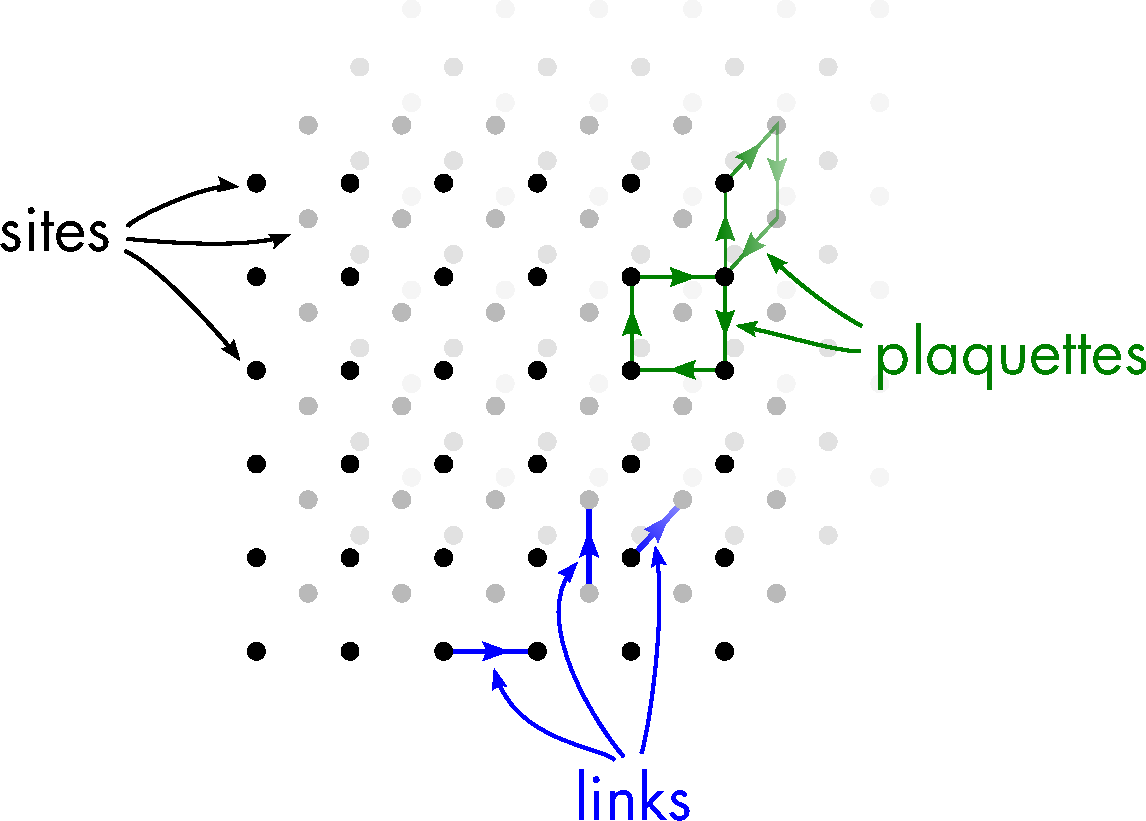
\includegraphics[width=0.9\textwidth]{figs/lattice-diagram}
\end{frame}

\begin{frame}{Partitioning a 3D lattice}
	\center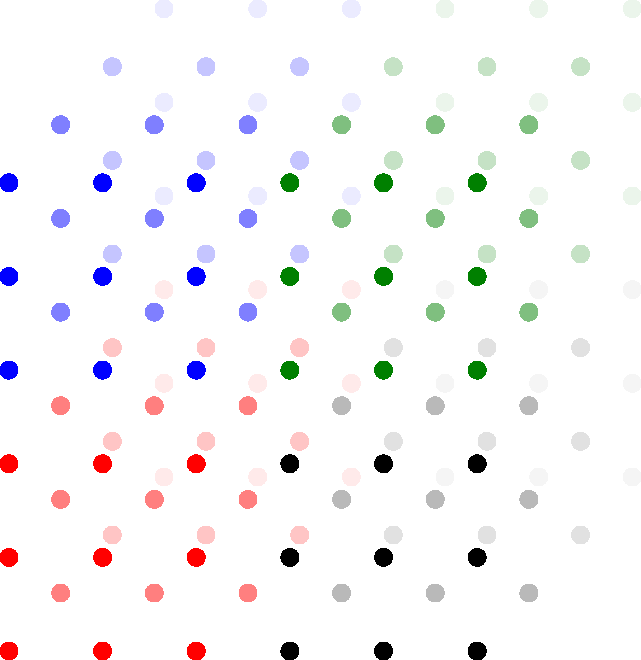
\includegraphics[width=0.53\textwidth]{figs/lattice-diagram-partition}
\end{frame}

\begin{frame}[fragile]{A quick refresher}
	\begin{itemize}[<+->]
		\item MPI: \textbf{M}essage \textbf{P}assing \textbf{I}nterface
		\item Born in 1991, now at version 3.1
		\item Single Program Multiple Data model
		\begin{itemize}[<+->]
			\item Same program runs multiple times (on one or more nodes)
			\item Communication is explicit
		\end{itemize}
		\item Initialise program with \verb|MPI_Init|, finish with \verb|MPI_Finalize|
		\item Point-to-point send and receive with \verb|MPI_Send|, \verb|MPI_Recv|
		\item \textbf{I}mmediate (non-blocking) versions: \verb|MPI_Isend|, \verb|MPI_Irecv|
		\item Point-to-all operations with \verb|MPI_Bcast|
		\item Collectives, e.g. \verb|MPI_Reduce|
	\end{itemize}
\end{frame}

\begin{frame}[fragile]{TIL \#3: \texttt{use mpi\_f08}}
	\begin{itemize}[<+->]
		\item Makes the \texttt{ierr} return variable \texttt{optional}
		\item Everything isn't an integer any more!
		\begin{itemize}[<+->]
			\item E.g. arguments of \verb|MPI_Wait| are now \verb|type(MPI_Request)| and \verb|type(MPI_Status)|
		\end{itemize}
		\item In-place reductions
		\begin{verbatim}
call MPI_AllReduce(MPI_In_Place, vel2, 1, MPI_Real, &
                   MPI_Sum, comm)\end{verbatim}
	\end{itemize}
\end{frame}

\begin{frame}[fragile]{TIL \#2: Subarray types}
  \noindent\small
  	\begin{verbatim}
subroutine init_single_halo_type_4(direction, position, size4, &
                                   datatype, typetarget)
  integer, intent(in) :: direction, position, size4
  type(MPI_Datatype), intent(in) :: datatype
  type(MPI_Datatype), intent(out) :: typetarget
  integer, dimension(4) :: sizes, subsizes, starts

  sizes = (/ ksizex_l + 2, ksizey_l + 2, ksizet_l + 2, size4 /)
  subsizes = (/ ksizex_l, ksizey_l, ksizet_l, size4 /)
  subsizes(direction+1) = 1
  starts = (/ 1, 1, 1, 0 /)
  starts(direction+1) = position

  call MPI_Type_Create_Subarray(4, sizes, subsizes, starts, &
                   MPI_Order_Fortran, datatype, typetarget)
  call MPI_Type_Commit(typetarget)
  return
end subroutine init_single_halo_type_4
\end{verbatim}

	
\end{frame}

\begin{frame}[fragile]{TIL \#1: MPI-IO}
	\begin{itemize}[<+->]
		\item Avoid channelling all I/O through a single rank/node
		\item Higher performance for reading and writing data
		\item Works really well with subarray types
	\end{itemize}\pause\small
	\begin{verbatim}
call MPI_File_Open(comm, 'con', MPI_Mode_Rdonly, &
                   MPI_Info_Null, mpi_fh)
call MPI_File_Set_View(mpi_fh, 0_8, MPI_Real, mpiio_type, &
                       "native", MPI_Info_Null)
call MPI_File_Read_All(mpi_fh, theta, &
                       3 * ksizex_l * ksizey_l * ksizet_l, &
                       MPI_Real, status)
call MPI_File_Close(mpi_fh)\end{verbatim}
\end{frame}

\begin{frame}[fragile]{TIL \#4: Cartesian communicators}
	\begin{itemize}[<+->]
		\item Give some structure to the set of processes
		\item Can be created with periodic boundaries
		\begin{verbatim}
call MPI_cart_create(MPI_COMM_WORLD, 3, &
                     (/ NP_X, NP_Y, NP_T /), &
                     (/ .true., .true., .true. /), &
                     .true., comm)\end{verbatim}
		\item Can access processes relative to current one:
		\begin{verbatim}call MPI_Cart_Shift(comm, 2, 1, ip_tdn, ip_tup)\end{verbatim}
		\begin{itemize}[<+->]
			\item Gives index of processes in both directions
		\end{itemize}
	\end{itemize}
\end{frame}

\begin{frame}[fragile]{TIL \#5: Persistent MPI communications}
	\begin{itemize}[<+->]
		\item Each \verb|MPI_Send|/\verb|MPI_Recv| pair has an overhead
		\item For a tight loop, this wastes time
		\item Instead, use \verb|MPI_Send_Init|/\verb|MPI_Recv_Init| outside the loop
		\item \verb|MPI_Start|/\verb|MPI_StartAll| inside
		\item Also need \verb|MPI_Wait|/\verb|MPI_WaitAll|
		\item Collectives planned for MPI 3.2, e.g. \verb|MPI_AllReduce_Init|
	\end{itemize}
\end{frame}

\begin{frame}{Step 1: Halos}
	\begin{itemize}[<+->]
		\item Add a 1-site border around all three dimensions
		\begin{itemize}[<+->]
			\item Only if $\phi_{i+1,j,k}$ is needed
		\end{itemize}
		\item Store contents of $\phi_{1,j,k}$ in $\phi_{n_x+1,j,k}$, $\phi_{n_x,j,k}$ in $\phi_{0,j,k}$, etc.
		\item Functions to update halos
		\begin{itemize}[<+->]
			\item Use a module -- \texttt{comms} -- for this
			\item Can then swap out for MPI version later
		\end{itemize}
		\item Test each function still gives same results as previously
	\end{itemize}
\end{frame}

\begin{frame}{Step 2: I/O}
	\begin{itemize}[<+->]
		\item Reimplement configuration read and write using MPI-IO
		\item Existing implementation saved RNG state in configuration
		\begin{itemize}[<+->]
			\item Store state from rank 0
			\item Reseed other ranks as \texttt{state + rank}
		\end{itemize}
		\item Check that read and write still give same results
	\end{itemize}
\end{frame}

\begin{frame}[fragile]{Step 3: Subarray type initialisation}
	\begin{itemize}[<+->]
		\item Add MPI initialisation function to set up MPI subarray types
		\item Separate types for each array shape, each boundary, each direction, each datatype
		\begin{itemize}[<+->]
			\item 4D (real and complex), 5D, 6D
			\item $x, y, t$; up, down; send, receive
			\item Varying sizes of 4th, 5th, 6th dimensions
			\item Use arrays for this
			\item Populate only required array elements
			\item e.g. \verb|size6| needs to be 1, 12, and 25; create \verb|halo_6_xdn_send(4:4, 1:25)|; populate elements 1, 12, 25
		\end{itemize}
		\item Include the type for MPI-IO here
	\end{itemize}
\end{frame}

\begin{frame}[fragile]{Step 4: Halo communication}
	\begin{itemize}[<+->]
		\item For each dimensionality, a function to do both \verb|MPI_Isend| and \verb|MPI_Irecv|
		\item Also takes in an array of \verb|MPI_Request|s and fills it
		\item A separate function to complete updates in any dimensionality
		\begin{itemize}[<+->]
			\item Only takes in an array of 12 \verb|MPI_Request| objects
		\end{itemize}
		\item Unit test
	\end{itemize}
\end{frame}

\begin{frame}[fragile]{Step 5: Parallelise most functions}
	\begin{itemize}[<+->]
		\item Replace global with local dimensions
		\item Before any function call relying on halos:
		\begin{itemize}[<+->]
			\item Work out where data last edited
			\item Add a halo update start at that point
			\item Complete update in time for its use
		\end{itemize}
		\item Any collective operation gets an \verb|MPI\_AllReduce|
		\item All MPI calls are wrapped with \verb|#ifdef MPI|
		\item Check regression tests
	\end{itemize}
\end{frame}

\begin{frame}{Step 6: Loose ends}
	\begin{itemize}[<+->]
		\item Correlation functions: lots of extra bookkeeping
		\item Reading input parameters: do on rank 0 and broadcast
	\end{itemize}
\end{frame}

\begin{frame}{Performance on Hawk}
	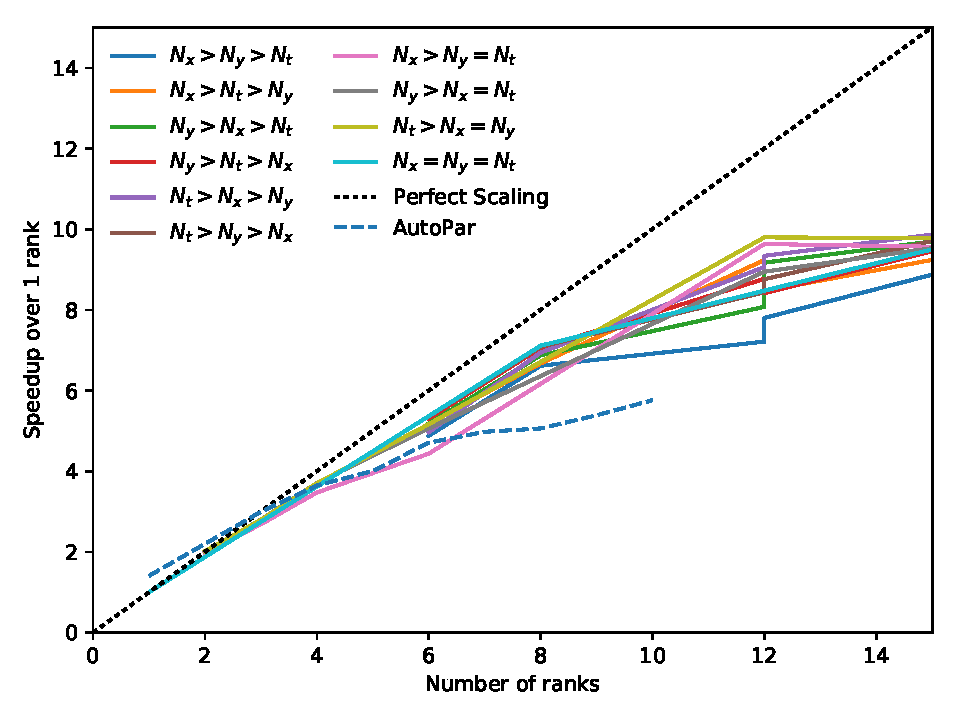
\includegraphics[width=\textwidth]{figs/scaling-hawk}
\end{frame}

\begin{frame}{Performance on Hawk}
	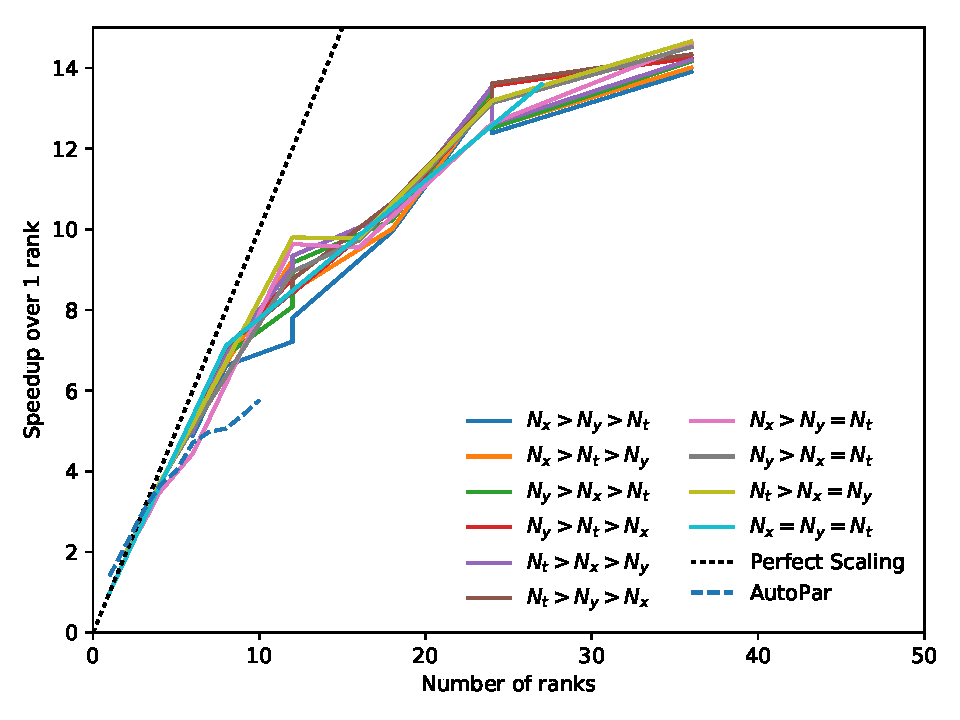
\includegraphics[width=\textwidth]{figs/scaling-hawk2}
\end{frame}

\begin{frame}{Weak and strong scaling of a single operation}
	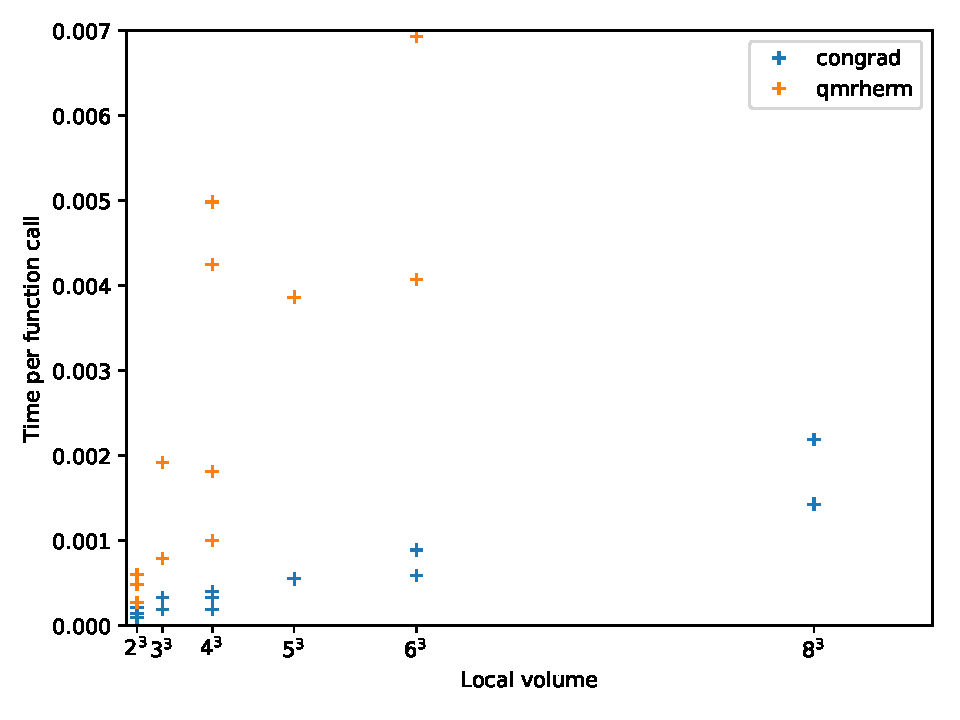
\includegraphics[width=\textwidth]{figs/precise}
\end{frame}

\begin{frame}[fragile]{Why doesn't it scale well past 8--12 processes?}
	\begin{itemize}[<+->]
		\item Try persistent send/receive?
		\begin{itemize}[<+->]
			\item Up to 20\% speedup on Broadwell+OPA
			\item No improvement on Skylake+Mellanox
			\item Persistent \verb|AllReduce| has to wait...
		\end{itemize}
		\item Noncontiguous send/receive regions?
		\begin{itemize}[<+->]
			\item ITAC shows \verb|MPI_Isend| takes time, which is weird
			\item Possibly due to data rearrangement
			\item Need to reintroduce indirection to fix this
		\end{itemize}
		\item Insufficient hiding of communication
		\begin{itemize}[<+->]
			\item Delay calls to \verb|MPI_Wait| until relevant work is reached
			\item Initial tests not promising - but only 10\% of work hidden
			\item Hiding more requires restructuring loops
			\item Significantly more mess
		\end{itemize}
	\end{itemize}
\end{frame}

\begin{frame}{Thanks for listening!}
	\Wider[0em]{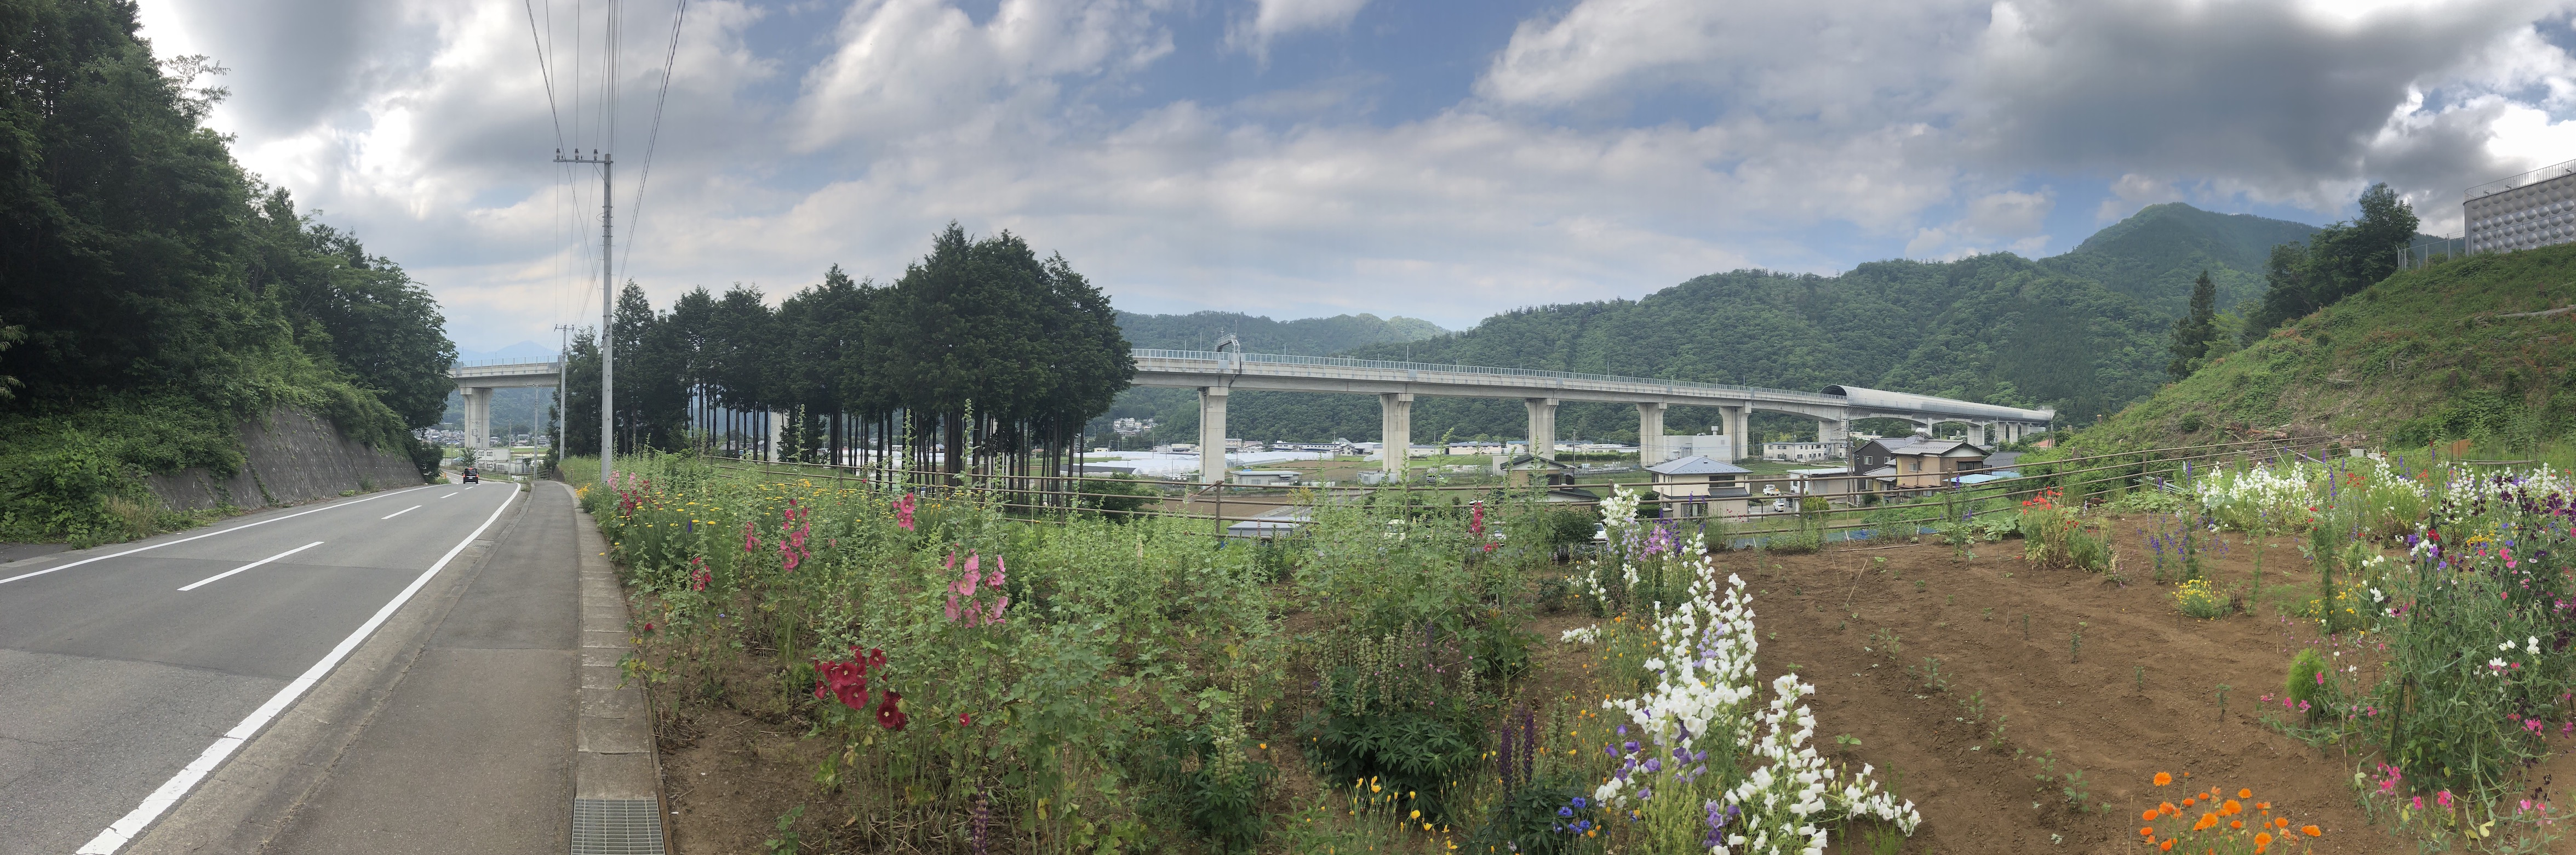
\includegraphics[width=\textwidth]{figs/maglev-panorama}}
\end{frame}

\end{document}
